\chapter{Introduction}
The growing interest of general public in those technologies that were 
research-only exclusives once, makes them cheaper and spread further and
animates research again.

The omnidirectional and full spherical cameras are perfect examples 
for this trend.
These devices have been used in robotics since their first appearance and they 
can be exploited in today consumer technologies like Augmented and Virtual 
Reality (AR/VR) devices and autonomous driving vehicles.

In this work we designed a \textit{Structure from Motion} (SfM) pipeline for 
full spherical cameras.

SfM is a well known topic in computer vision, it addresses the problem of 
recovering the structure of the 3D environments from a sequence of images taken 
from different point of views.

Most of the work about SfM, and computer vision in general, 
has targeted perspective cameras, since these type of devices 
have always been more common.
With the increased diffusion of panoramic cameras, the interest to use them in 
various computer vision topics increased too.

\section{Benefits of Full Spherical Cameras}
Because of the increased \textit{Field of View} (FoV), panoramic cameras can 
capture a larger amount of data compared to traditional devices.
The two fisheye lenses in the Ricoh Theta allow us to utilize also rear 
correspondences between images and this may improve the motion 
estimation performances.

Another advantage of full spherical cameras is that they do not require 
a calibration phase for intrinsic parameters estimation. 
Camera calibration is an essential requirement for most computer vision 
applications,
it aims to estimate several parameters, like focal length, image 
sensor size, pixel density and lens distortions. When dealing with full 
spherical cameras, we can assume the image is produced on a unitary sphere 
therefore we can set the focal length to 1.
Further details about 
the camera model and the parameters involved can be found in 
chapter \ref{ch:state_of_the_art}.

\section{SfM, VO and SLAM}
\textit{Structure from Motion} is a long studied topic in computer vision; 
it is about estimating camera poses and 
reconstructing the 3D environment captured by the 
pictures of those cameras.
Some of the first work in this field are the paper by Longuet-Higgins 
(\cite{longuet1981computer}) whose equation is fundamental in epipolar geometry,
and by Tomasi et al. who used an orthographic pictures to estimate a 3D object 
in \cite{tomasi1992shape}.

SfM is a general term that includes \textit{Visual Odometry} (VO). This is 
the problem of recovering the motion of an agent equipped with a camera rig in 
a 3D environment. VO usually deals with an ordered set of images, like a video 
stream, and uses them to compute the egomotion in real time.
The term \textit{visual odometry} was first introduces by Nister et al. 
in \cite{nister2004visual}.

Another field of robotic research that is very close to the objective of VO is
\textit{Simultaneous Localization And Mapping} (SLAM) which target the problem 
of creating a map of the environment where a camera equipped agent navigates 
and estimating its path.
As Scaramuzza says in \cite{scaramuzzaVisualOdometryI}, while VO is more 
focused on local motion estimation, SLAM's goal is to obtain a global 
consistent estimation of the agent movements.
In order to reduce error, SLAM keeps track of the visited path and is able to 
decide when the agent comes back to a previously visited location.
This extra step in SLAM's pipeline is called \textit{loop closure} and provides 
an additional constraint used to reduce errors in both the agent's path and 
environment reconstruction.
The term SLAM was introduced by Durrant-White et al. in 
\cite{durrant1996localization}.

\section{Omnidirectional and Full Spherical Cameras}
\label{sec:cameraclassification}
Omnidirectional cameras are characterized by wide field of view, 
indeed many of this kind
of devices can take pictures with a 180\degree view angle or even wider.

There are several ways to obtain panoramic images, they include:
\begin{itemize}
	\item perspective cameras and image stitching;
	\item catadioptric cameras;
	\item dioptric cameras;
	\item hybrid approaches.
\end{itemize}

Perspective cameras can take panoramic pictures with the aid of 
software stitching: first, we take several pictures with many cameras or by
simply moving 
the same camera in order to cover a larger scene. Then the stitching software 
creates a single picture out of the set of images.
The single perspective camera and the stitching software is the cheapest 
way to obtain panoramic images because it does not need any kind of specialized 
hardware. However it is impossible to record videos since the shooting phase 
requires time.

Catadioptric cameras are obtained with a perspective camera and a mirror 
mounted in front of it. 
The camera take a picture of the mirror which reflects the the 
surrounding. The mirror of a catadioptric system may have several shapes, 
although a common one is the hyperbolic profile that creates a single center of 
projection for every ray coming to the mirror.

A traditional camera can also be adapted to work as a panoramic one by adding
fisheye lenses capable of refracting lights from wide angle towards the 
image sensor. This setup are called dioptric cameras.

Apart of perspective cameras coupled with stitching software, none of the 
previous approach can take full spherical panoramic photos, while full spherical 
videos can not be shot with perspective cameras either.
The fourth approach, the hybrid one, exploits several fisheye lenses and 
software stitching to capture full spherical panoramic images in a single shot, 
thus enabling full spherical video capturing as well.
The camera (that is composed of several image sensors) take multiple 
overlapping pictures simultaneously, then the stitching software composes the
data in a single image.

In all our experiments we used the Ricoh Theta S camera 
(see Fig. \ref{fig:ricoh_theta}) which is a hybrid full spherical camera 
composed of two fisheye lenses with a FOV greater than 180\degree.
\begin{figure}
\centering
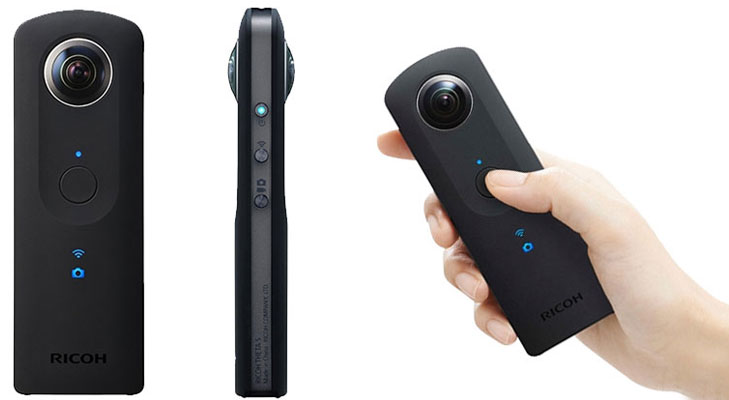
\includegraphics[width=0.7\textwidth]{img/theta_s}
\label{fig:ricoh_theta}
\caption{The Ricoh Theta S 360\degree camera}
\end{figure}
\todo{Puo' bastare citare la fonte dell'immagine per utilizzarla nella tesi?}

